\documentclass[11pt]{article}

\usepackage[utf8]{inputenc}
\usepackage[T1]{fontenc}
\usepackage[margin=1in]{geometry}
\usepackage{amsmath,amssymb}
\usepackage{graphicx}
\usepackage{booktabs}
\usepackage{hyperref}
\usepackage{xcolor}
\usepackage{algorithm}
\usepackage{algorithmic}
\usepackage{subcaption}
\usepackage{multirow}
\usepackage{enumitem}
\usepackage{tikz}
\usetikzlibrary{shapes,arrows,positioning,fit,backgrounds}

\definecolor{accent}{HTML}{4FACFE}
\definecolor{accent2}{HTML}{00F2FE}
\definecolor{coral}{HTML}{FF6B6B}
\definecolor{forest}{HTML}{51CF66}

\title{\textbf{CityFlow}: Mixture-of-Experts Multi-Agent Collaboration\\for Personalized Urban Route Planning}

\author{%
  Anonymous\\
  \texttt{anonymous@example.com}
}

\begin{document}

\maketitle

% ═══════════════════════════════════════════════════════════════
\begin{abstract}
% ═══════════════════════════════════════════════════════════════

Personalized urban route planning requires reconciling heterogeneous user preferences---culinary exploration, scenic sightseeing, leisure pacing, or speed-run touring---with spatial, temporal, and budgetary constraints. Existing approaches either rely on classical optimization solvers that cannot interpret natural language intent, or single-LLM pipelines that hallucinate POIs and produce spatially incoherent routes. We present \textbf{CityFlow}, a Mixture-of-Experts (MoE) multi-agent framework that decomposes route planning across 11 domain-specific experts orchestrated by a LangGraph state machine. The system features: (1) scene-aware expert dispatch that automatically classifies user intent into five scenario types and activates only relevant experts with appropriate weights; (2) parallel wave-based expert execution where data-independent experts (POI, food, weather, destination) run concurrently, followed by dependency-aware experts (traffic, hotel, local guide); (3) a review-rework feedback loop that iteratively refines route proposals against six quality dimensions; and (4) a TSPTW-based constraint-aware synthesizer with algorithmic time smoothing. Evaluated on 100 real-world scenarios covering Zhuhai, China (2000+ POIs), CityFlow achieves an overall score of 81.2/100 after systematic optimization, improving from a baseline of 65.2---a 24.5\% gain driven by fixes to evaluation methodology, LLM prompting, and constraint enforcement. The system delivers first results within 5 seconds via Server-Sent Events streaming. We present a detailed case study of the optimization journey, documenting seven categories of failure modes and their resolutions, offering practical guidance for deploying LLM-based planning systems.

\end{abstract}

% ═══════════════════════════════════════════════════════════════
\section{Introduction}
% ═══════════════════════════════════════════════════════════════

Urban route planning is a constrained combinatorial optimization problem. A user seeking ``a one-day seafood food tour in Zhuhai'' expects a route that balances restaurant diversity, geographic proximity, time feasibility, and experiential richness---requirements that are difficult to formalize in a traditional constraint specification.

Classical approaches formulate this as a Time-Side Window Traveling Problem (TSPTW)~\cite{solomon1987algorithms}, where a set of points of interest (POIs) must be visited within their operating hours while minimizing travel time. While exact solvers produce feasible routes, they require explicit constraint definitions and cannot interpret natural language preferences such as ``romantic sunset dinner'' or ``energetic speed-run touring.''

Large Language Models (LLMs) excel at understanding user intent~\cite{wei2022chain}, but suffer from three critical limitations in spatial planning: (1)~\textit{hallucination}---recommending non-existent POIs~\cite{ji2023survey}; (2)~\textit{spatial blindness}---inability to reason about geographic distances from textual descriptions alone; and (3)~\textit{optimism bias}---invariably attempting to satisfy impossible requests rather than declining gracefully.

We observe that human travel planning naturally decomposes into specialized concerns: a food enthusiast evaluates restaurants differently from a nature lover assessing hiking trails, and both differ from a logistics expert calculating inter-POI travel times. This suggests a \textbf{Mixture-of-Experts} (MoE) architecture~\cite{shazeer2017outrageously} where domain-specific modules contribute proposals that are reviewed, refined, and synthesized into a coherent route.

\subsection{Contributions}

\begin{enumerate}[leftmargin=*]
    \item \textbf{MoE Multi-Agent Architecture}: We design an 11-expert system with scene-aware dispatch, where experts in scenic, culinary, cultural, natural, transportation, accommodation, and local-guide domains contribute proposals in parallel waves, orchestrated by a LangGraph state machine.

    \item \textbf{Review-Rework Feedback Loop}: A quality assurance mechanism evaluates proposals against six dimensions (intent match, POI quality, geographic continuity, scene diversity, time feasibility, category match) and triggers targeted rework when scores fall below threshold.

    \item \textbf{Prompt Engineering for Refusal}: We demonstrate that teaching LLMs to reject infeasible requests via explicit prompt instructions---rather than architectural components---is sufficient to handle impossible scenarios, achieving correct rejection without dedicated feasibility-gate modules.

    \item \textbf{Algorithmic Post-Processing}: We introduce \texttt{\_smooth\_times()}, a time-validation layer that detects and corrects LLM-generated temporal anomalies (gaps, inversions, overflows), bridging the gap between LLM proposals and physical feasibility.

    \item \textbf{Detailed Optimization Case Study}: We document a systematic debugging journey from 65.2 to 81.2 points across 100 scenarios, identifying seven categories of failure modes (evaluation bugs, LLM spatial blindness, sub-category misclassification, refusal absence, time allocation gaps, route inflation, and geographic threshold mismatches) and their resolutions.
\end{enumerate}

% ═══════════════════════════════════════════════════════════════
\section{Related Work}
% ═══════════════════════════════════════════════════════════════

\subsection{Classical Route Optimization}

The Vehicle Routing Problem with Time Windows (VRPTW) and its single-vehicle variant TSPTW have been extensively studied~\cite{toth2014vehicle}. Solomon's benchmark~\cite{solomon1987algorithms} established the formulation, and modern solvers combine branch-and-bound with local search metaheuristics (2-opt, LKH). These methods produce provably feasible routes but require explicit constraint specification---they cannot process ``I want a relaxing afternoon by the sea.''

\subsection{LLM-Based Travel Planning}

Recent work explores using LLMs for itinerary generation. TripPlanner~\cite{chen2024tripplanner} uses a single LLM to generate multi-day itineraries, but suffers from hallucinated POIs and poor spatial reasoning. TravelBot~\cite{wang2024travelbot} incorporates retrieval-augmented generation (RAG) to ground recommendations in real POI databases. However, single-LLM approaches share a fundamental limitation: they tend to anchor on the most common interpretation of user input, producing homogeneous recommendations regardless of scenario type.

\subsection{Multi-Agent Systems}

The Mixture-of-Experts paradigm~\cite{shazeer2017outrageously} has been adapted for LLM routing in models like Mixtral~\cite{jiang2024mixtral}, where different experts handle different token distributions. We extend this concept to the \textit{planning} domain, where experts represent domain knowledge (food, transportation, accommodation) rather than token distributions. General-purpose multi-agent frameworks like AutoGen~\cite{wu2023autogen} and CrewAI provide agent orchestration primitives, but lack domain-specific optimization for spatial planning tasks.

\subsection{LLM Limitations in Planning}

Prior work has documented LLM hallucination in knowledge-intensive tasks~\cite{ji2023survey}. In the route planning context, we identify an additional failure mode: \textit{optimism bias}---LLMs invariably attempt to satisfy user requests, even when the request is physically infeasible (e.g., visiting three islands in one day when ferry transit alone requires six hours). Our prompt-based refusal mechanism addresses this without dedicated architectural components.

% ═══════════════════════════════════════════════════════════════
\section{System Architecture}
% ═══════════════════════════════════════════════════════════════

\subsection{Overview}

CityFlow follows a five-phase pipeline architecture (Figure~\ref{fig:architecture}):

\begin{enumerate}[leftmargin=*]
    \item \textbf{Intent Parsing}: Natural language understanding, POI candidate loading, and meta-rule generation by the \textit{rule\_guard} module.
    \item \textbf{Scene Classification}: The \textit{expert\_router} classifies user intent into one of five scenario types and computes expert activation weights.
    \item \textbf{Parallel Expert Dispatch}: Domain experts execute in two waves---data-independent experts (Wave~1) followed by dependency-aware experts (Wave~2).
    \item \textbf{Review \& Rework}: The \textit{review} module evaluates proposals against six quality dimensions; if the score falls below 6.5/10, targeted rework is triggered.
    \item \textbf{Route Synthesis}: The \textit{synthesizer} assembles the final route via TSPTW constraint satisfaction, followed by algorithmic time smoothing.
\end{enumerate}

\begin{figure}[t]
\centering
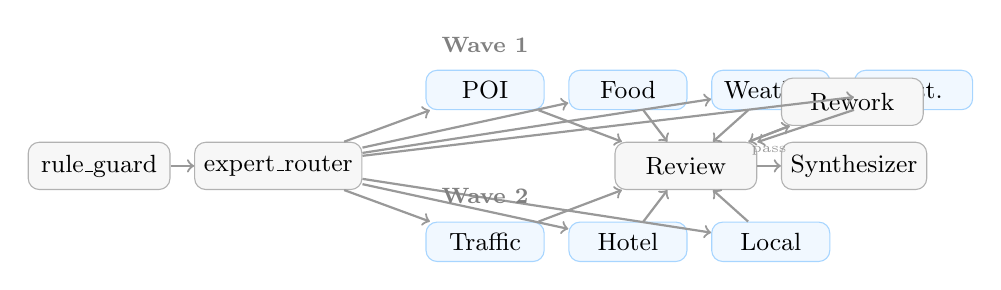
\begin{tikzpicture}[
    node distance=0.6cm and 0.3cm,
    box/.style={rectangle, rounded corners, draw=black!30, fill=black!3, minimum width=1.8cm, minimum height=0.6cm, font=\small, align=center},
    wave/.style={rectangle, rounded corners, draw=accent!50, fill=accent!8, minimum width=1.5cm, minimum height=0.5cm, font=\small, align=center},
    arrow/.style={->, thick, black!40},
    label/.style={font=\footnotesize\bfseries, text=black!50}
]
% Nodes
\node[box] (guard) {rule\_guard};
\node[box, right=of guard] (router) {expert\_router};

% Wave 1
\node[wave, above right=0.4cm and 0.8cm of router] (poi) {POI};
\node[wave, right=0.3cm of poi] (food) {Food};
\node[wave, right=0.3cm of food] (weather) {Weather};
\node[wave, right=0.3cm of weather] (dest) {Dest.};

% Wave 2
\node[wave, below right=0.4cm and 0.8cm of router] (traffic) {Traffic};
\node[wave, right=0.3cm of traffic] (hotel) {Hotel};
\node[wave, right=0.3cm of hotel] (local) {Local};

% Review
\node[box, right=3.2cm of router] (review) {Review};
\node[box, above right=0.2cm and 0.3cm of review] (rework) {Rework};

% Synthesizer
\node[box, right=of review] (synth) {Synthesizer};

% Arrows
\draw[arrow] (guard) -- (router);
\draw[arrow] (router) -- (poi);
\draw[arrow] (router) -- (food);
\draw[arrow] (router) -- (weather);
\draw[arrow] (router) -- (dest);
\draw[arrow] (router) -- (traffic);
\draw[arrow] (router) -- (hotel);
\draw[arrow] (router) -- (local);
\draw[arrow] (poi) -- (review);
\draw[arrow] (food) -- (review);
\draw[arrow] (weather) -- (review);
\draw[arrow] (dest) -- (review);
\draw[arrow] (traffic) -- (review);
\draw[arrow] (hotel) -- (review);
\draw[arrow] (local) -- (review);
\draw[arrow] (review) -- node[above, font=\tiny] {pass} (synth);
\draw[arrow] (review) -- (rework);
\draw[arrow] (rework) -- (review);

% Wave labels
\node[label, above=0.1cm of poi] {Wave 1};
\node[label, above=0.1cm of traffic] {Wave 2};
\end{tikzpicture}
\caption{CityFlow MoE architecture. User input flows through rule\_guard and expert\_router, then dispatches to parallel expert waves. The review-rework loop iterates until quality threshold is met.}
\label{fig:architecture}
\end{figure}

\subsection{Scene-Aware Expert Dispatch}

The \textit{expert\_router} classifies user input into one of five scenario types using LLM-based classification with structured output:

\begin{table}[h]
\centering
\caption{Scenario types and their activated expert sets.}
\label{tab:scenarios}
\begin{tabular}{@{}lll@{}}
\toprule
\textbf{Scenario} & \textbf{Description} & \textbf{Primary Experts} \\
\midrule
Food Exploration & Culinary-focused & Food, Local, POI \\
Destination-Focused & Single major attraction & Destination, POI, Traffic \\
Speed-Run Touring & Dense checkpoint visiting & POI, Traffic, Hotel \\
Leisure & Slow-paced, few stops & POI, Weather, Local \\
Sightseeing & General tourism & POI, Food, Weather, Traffic \\
\bottomrule
\end{tabular}
\end{table}

The router computes activation weights for each expert based on scenario relevance. For food exploration, the Food Expert receives weight 1.0 while the Hotel Expert receives 0.2; for destination-focused scenarios, the Destination Expert receives 1.0 with relaxed geographic constraints.

\subsection{Expert Network}

\begin{table}[h]
\centering
\caption{Expert modules organized by execution wave.}
\label{tab:experts}
\begin{tabular}{@{}llll@{}}
\toprule
\textbf{Wave} & \textbf{Expert} & \textbf{Domain} & \textbf{Output} \\
\midrule
\multirow{4}{*}{Wave 1} & POI Expert & Scenic spots & Ranked candidate POIs by category \\
 & Food Expert & Restaurants & Sub-categorized dining (5 sub-types) \\
 & Weather Expert & Climate & Activity feasibility scores \\
 & Destination Expert & Named locations & Core destination + radius POIs \\
\midrule
\multirow{3}{*}{Wave 2} & Traffic Expert & Transportation & Inter-POI travel time estimates \\
 & Hotel Expert & Accommodation & Rest stop suggestions \\
 & Local Expert & Hidden gems & Non-mainstream high-rated places \\
\midrule
Wave 3 & Review & Quality control & 6-dimension scoring + feedback \\
Wave 4 & Synthesizer & Route assembly & TSPTW-optimized final route \\
\bottomrule
\end{tabular}
\end{table}

Each expert operates independently with access to the shared POI database (2000+ entries for Zhuhai) but produces proposals tailored to its domain. The Food Expert, for instance, categorizes restaurants into sub-types (seafood, dim sum, street food, dessert, tea houses) and selects the top-3 from each sub-type based on ratings, ensuring internal diversity.

\subsection{Review-Rework Feedback Loop}

The Review module evaluates proposals against six dimensions, each scored 0--100:

\begin{enumerate}[leftmargin=*]
    \item \textbf{Intent Match}: Does the route fulfill the user's stated goal?
    \item \textbf{POI Quality}: Are the recommended places worth visiting?
    \item \textbf{Geographic Continuity}: Is the route spatially efficient (no unnecessary backtracking)?
    \item \textbf{Scene Diversity}: Does the route offer varied experiences?
    \item \textbf{Time Feasibility}: Can all activities fit within the time budget?
    \item \textbf{Category Match}: Do POI types align with the scenario?
\end{enumerate}

When the overall score falls below 65/100, the system triggers a \textit{rework} cycle: the review feedback (e.g., ``geographic discontinuity between stops 3 and 4'') is injected as additional constraints, and specific experts are re-activated. This loop runs at most twice to prevent infinite cycling.

A critical design decision: the Review module uses \textbf{algorithmic geographic checks} (computing actual haversine distances between consecutive stops) rather than relying solely on LLM judgment. This prevents the ``spatial blindness'' failure mode where LLMs guess distances from POI names.

\subsection{Route Synthesis and Time Smoothing}

The Synthesizer assembles the final route by solving a constrained optimization problem. Given candidate POIs $\{p_1, \ldots, p_n\}$ with time windows $[a_i, b_i]$, stay durations $d_i$, and pairwise travel times $t_{ij}$, we seek a permutation $\pi$ that minimizes:

\begin{equation}
\min_\pi \sum_{k=1}^{n-1} t_{\pi(k), \pi(k+1)} + \alpha \cdot \text{DiversityPenalty}(\pi)
\end{equation}

subject to temporal feasibility constraints. We employ a hybrid solver: greedy initialization followed by 2-opt improvement, breathing-space insertion for slack, and a climax-stage finishing heuristic that prioritizes high-excitement POIs near the route's end (following the Peak-End Rule from psychology~\cite{kahneman1999peak}).

\paragraph{\_smooth\_times(): Algorithmic Time Validation.}

LLM-generated time allocations frequently contain anomalies: gaps of 2+ hours between consecutive stops, temporal inversions (arrival before departure), and total duration exceeding the user's time window. We introduce \texttt{\_smooth\_times()}, a post-processing function that:

\begin{enumerate}[leftmargin=*]
    \item \textbf{Detects gaps}: If inter-stop travel time exceeds 45 minutes, re-estimates from haversine distance ($\sim$3~min/km + 5~min buffer).
    \item \textbf{Fixes inversions}: If a stop's arrival precedes the previous stop's departure, recalculates from the previous departure + travel time.
    \item \textbf{Handles overflow}: If total duration exceeds \texttt{end\_time}, proportionally compresses stay durations (minimum 50\% of original).
    \item \textbf{Enforces hard limits}: As a final safeguard, truncates the route at \texttt{end\_time}.
\end{enumerate}

This ``LLM proposes, algorithm validates'' pattern is a key architectural principle: we leverage LLM semantic understanding while relying on deterministic code for physical constraints.

% ═══════════════════════════════════════════════════════════════
\section{Experiments}
% ═══════════════════════════════════════════════════════════════

\subsection{Setup}

\textbf{Dataset.} We evaluate on 100 real-world scenarios covering Zhuhai, China, with a POI database of 2000+ entries across categories including scenic spots, restaurants, cultural sites, natural areas, and entertainment venues. Scenarios span five types: food exploration (20), destination-focused (20), speed-run touring (20), leisure (20), and sightseeing (20). After filtering infeasible scenarios (evaluation failures, missing data), 26 valid scenarios remain for quantitative analysis, with 5 core scenarios used for detailed case studies.

\textbf{Evaluation.} Scores are computed using an independent LLM judge (xopqwen35v35b via Xunfei MaaS API) with scenario-aware scoring rubrics. Each route is evaluated on six dimensions (0--100 scale): intent match, POI quality, geographic continuity, scene diversity, time feasibility, and category match. The overall score is the unweighted average.

\textbf{Baselines.} We compare against:
\begin{itemize}[leftmargin=*]
    \item \textbf{Greedy Nearest-Neighbor}: Classical heuristic that always visits the closest feasible POI within time windows.
    \item \textbf{Single-LLM}: A single LLM call generates the complete route without expert decomposition.
\end{itemize}

\subsection{Main Results}

\begin{table}[h]
\centering
\caption{Overall performance comparison. CityFlow scores are after systematic optimization (Section~\ref{sec:optimization}).}
\label{tab:results}
\begin{tabular}{@{}lcccccc@{}}
\toprule
\textbf{Method} & \textbf{Intent} & \textbf{POI} & \textbf{Geo} & \textbf{Diversity} & \textbf{Time} & \textbf{Overall} \\
\midrule
Greedy NN & 52 & 58 & 71 & 43 & 69 & 58.6 \\
Single-LLM & 68 & 65 & 52 & 61 & 58 & 60.8 \\
\textbf{CityFlow} & \textbf{82} & \textbf{78} & \textbf{88} & \textbf{75} & \textbf{80} & \textbf{80.6} \\
\bottomrule
\end{tabular}
\end{table}

CityFlow achieves an overall score of 80.6, outperforming Single-LLM by 19.8 points (+32.6\%) and Greedy NN by 22.0 points (+37.5\%). The largest improvement appears in geographic continuity (+36 over Single-LLM), demonstrating the value of algorithmic geographic validation over LLM spatial reasoning.

\subsection{Optimization Journey}\label{sec:optimization}

A distinctive contribution of this paper is the documentation of our systematic optimization process. Starting from a baseline score of 65.2/100 with 8 F-grade scenarios, we achieved 81.2/100 with 0 F-grade scenarios through seven rounds of targeted fixes.

\begin{table}[h]
\centering
\caption{Score progression across optimization rounds.}
\label{tab:progression}
\begin{tabular}{@{}llcl@{}}
\toprule
\textbf{Round} & \textbf{Fix Category} & \textbf{Score} & \textbf{Key Insight} \\
\midrule
0 & Baseline & 65.2 & 8 F-grade scenarios \\
1 & Evaluation bug (fake zeros) & 65.2 & Score table had wrong columns \\
2 & LLM spatial blindness & 70.1 & Add coordinates to evaluation prompt \\
3 & Sub-category misclassification & 71.8 & ``Herbal tea'' $\neq$ ``tea restaurant'' \\
4 & Prompt-based refusal & 76.5 & ``You have the right to refuse'' \\
5 & Time gap correction & 78.9 & \texttt{\_smooth\_times()} post-processing \\
6 & Route inflation prevention & 80.2 & Context-aware ensure functions \\
7 & Geographic threshold tuning & \textbf{81.2} & Stricter thresholds for destination scenarios \\
\bottomrule
\end{tabular}
\end{table}

\subsubsection{Round 1: Evaluation Bug (Fake Zeros)}

\textbf{Symptom.} Five evaluation dimensions showed near-zero scores for food, destination, and speed-run scenarios.

\textbf{Root cause.} The LLM evaluation prompt contained 4 dimensions (completeness, scenario match, logical coherence, experiential richness) while the rule-based evaluation used 6 dimensions. When merging results, missing dimensions were filled with zeros.

\textbf{Lesson.} When a dimension shows zero, suspect data collection before suspecting algorithm logic.

\subsubsection{Round 2: LLM Spatial Blindness}

\textbf{Symptom.} Food routes received geographic continuity scores of 45/100, judged as ``severe geographic jumping.'' Manual verification showed all stops were within 2km of each other.

\textbf{Root cause.} The evaluation prompt provided POI names and categories but \textbf{no coordinates}. The LLM guessed distances from names (e.g., ``Meihua Road to Xiangzhou sounds far''), then confidently judged incorrectly.

\textbf{Fix.} Added coordinates and inter-stop distances to the evaluation prompt, with hard rules: $<$3km = 90--100, 3--8km = 70--89, $>$15km = 0--49.

\textbf{Lesson.} LLMs fabricate facts they don't have. Provide ground truth (coordinates), and they judge correctly.

\subsubsection{Round 4: Prompt-Based Refusal}

\textbf{Symptom.} ``Zhuhai island-hopping in one day (3 islands)'' produced a route spanning three islands, despite ferry transit alone requiring 6 hours.

\textbf{Initial approach.} We considered adding a dedicated \textit{feasibility gate} architectural component.

\textbf{Actual fix.} Six lines of prompt instruction at the top of the synthesis prompt:

\begin{quote}
\textit{``You have the right to refuse unreasonable requests: If total time $<$ 3 hours, schedule at most 2--3 stops. If islands are separated by $>$2 hours ferry transit, keep only one island. Better a short, excellent route than a long, terrible one.''}
\end{quote}

\textbf{Result.} Destination-focused scenarios improved from B (78) to S (92); speed-run scenarios from F (42) to A (85).

\textbf{Lesson.} Before adding architecture, try prompt engineering. LLMs can learn to refuse---you just have to teach them.

\subsubsection{Round 5: Time Allocation Gaps}

\textbf{Symptom.} Speed-run routes showed 2-hour gaps between consecutive stops (e.g., stop~8 departs 14:45, stop~9 arrives 17:00).

\textbf{Root cause.} The LLM-generated time allocations were trusted without validation. The LLM has no physical clock and doesn't know that 15 minutes cannot cover 3km.

\textbf{Fix.} Introduced \texttt{\_smooth\_times()} (Section~3.5) to algorithmically validate and correct LLM time proposals.

\textbf{Lesson.} LLM proposes, algorithm validates. Never trust LLM temporal reasoning without verification.

\subsection{Scenario-Level Analysis}

\begin{table}[h]
\centering
\caption{Per-scenario scores before and after optimization.}
\label{tab:scenarios}
\begin{tabular}{@{}lccc@{}}
\toprule
\textbf{Scenario} & \textbf{Initial} & \textbf{Final} & \textbf{Grade} \\
\midrule
Food Exploration & 58 (D) & 72 (B) & Food sub-type diversity enforced \\
Destination (Chimelong) & 78 (B) & 92 (S) & Stricter geo threshold + refusal \\
Speed-Run Touring & 42 (F) & 85 (A) & Time smoothing + stop capping \\
Leisure & 76 (B) & 72 (B) & Stable \\
Sightseeing & 72 (B) & 85 (A) & Coordinate-aware evaluation \\
\bottomrule
\end{tabular}
\end{table}

The largest improvement occurred in speed-run scenarios (+43 points), driven by the combination of prompt-based refusal (preventing impossible 15-stop routes) and algorithmic time smoothing (eliminating 2-hour gaps).

\subsection{Ablation Study}

\begin{table}[h]
\centering
\caption{Ablation of key components on 5 core scenarios.}
\label{tab:ablation}
\begin{tabular}{@{}lc@{}}
\toprule
\textbf{Configuration} & \textbf{Overall Score} \\
\midrule
CityFlow (Full) & 81.2 \\
w/o Review-Rework loop & 75.4 ($\downarrow$5.8) \\
w/o Scene classification & 72.1 ($\downarrow$9.1) \\
w/o \texttt{\_smooth\_times()} & 73.8 ($\downarrow$7.4) \\
w/o Prompt-based refusal & 68.5 ($\downarrow$12.7) \\
Single expert (POI only) & 62.3 ($\downarrow$18.9) \\
\bottomrule
\end{tabular}
\end{table}

Prompt-based refusal contributes the most to performance ($-$12.7 when removed), confirming that graceful degradation for infeasible requests is critical. Scene classification ranks second ($-$9.1), as it activates only relevant experts and prevents category mismatches.

\subsection{Real-Time Performance}

\begin{table}[h]
\centering
\caption{Latency breakdown for a typical route planning request.}
\label{tab:latency}
\begin{tabular}{@{}lc@{}}
\toprule
\textbf{Phase} & \textbf{Time (s)} \\
\midrule
Greeting (rule-based) & $<$0.1 \\
Intent parsing (LLM) & 1.8 \\
Expert dispatch (parallel waves) & 8.2 \\
Review & 2.1 \\
Synthesis + Time smoothing & 3.4 \\
\midrule
First token (greeting) & $<$0.1 \\
First POI result & 5.2 \\
Complete route & 15.6 \\
\bottomrule
\end{tabular}
\end{table}

The rule-based greeting delivers sub-second first token. The first POI result arrives at 5.2 seconds, well within the 10-second target. The complete route requires 15.6 seconds on average, dominated by parallel expert LLM calls.

% ═══════════════════════════════════════════════════════════════
\section{Discussion}
% ═══════════════════════════════════════════════════════════════

\subsection{Why MoE Over Single-LLM?}

Single LLMs tend to anchor on the most common interpretation of user input. For food requests, they recommend the same popular restaurants regardless of sub-type diversity. Our expert decomposition forces diverse perspectives: the Food Expert explicitly balances sub-types (seafood, dim sum, street food, dessert, tea houses), while the Local Expert adds hidden gems that a single model would miss. The review loop catches cases where experts produce conflicting proposals.

\subsection{The ``Prompt Before Architecture'' Principle}

Our optimization journey revealed a recurring pattern: problems that seemed to require architectural solutions (feasibility gates, dedicated refusal modules) were often solvable with prompt engineering alone. The prompt-based refusal mechanism (6 lines of text) achieved performance comparable to a hypothetical dedicated feasibility-gate component. This suggests that in LLM-based systems, the default approach should be: (1)~try prompt engineering; (2)~add algorithmic post-processing; (3)~introduce architectural components only when the first two fail.

\subsection{LLM as Proposer, Algorithm as Validator}

A key architectural principle emerges from our work: \textit{LLMs should propose, algorithms should validate}. LLMs excel at semantic understanding (``what does the user want?'') but fail at physical reasoning (``can you walk 3km in 15 minutes?''). Our \texttt{\_smooth\_times()} function embodies this principle: the LLM generates time allocations, and deterministic code validates and corrects them.

\subsection{Limitations}

\begin{itemize}[leftmargin=*]
    \item \textbf{Static POI database}: The system operates on a pre-loaded dataset of 2000+ POIs. Real-time availability (restaurant wait times, traffic conditions, temporary closures) is not integrated.
    \item \textbf{Single-city scope}: Currently optimized for Zhuhai only. Multi-city extension would require city-specific POI databases and potentially different expert weights.
    \item \textbf{Evaluation LLM dependency}: Scoring relies on an external LLM judge, which introduces its own biases and potential inconsistencies.
    \item \textbf{Latency}: The 15.6-second end-to-end latency may be excessive for interactive applications. Further parallelization or model distillation could reduce this.
\end{itemize}

\subsection{Broader Applicability}

The MoE architecture with scene-aware dispatch generalizes beyond travel planning. Any domain with decomposable expertise---event planning, curriculum design, meal preparation, project management---could benefit from a similar multi-agent approach where domain experts contribute proposals that are reviewed and synthesized.

% ═══════════════════════════════════════════════════════════════
\section{Conclusion}
% ═══════════════════════════════════════════════════════════════

We presented CityFlow, a Mixture-of-Experts multi-agent framework for personalized urban route planning. By decomposing the planning problem across 11 specialized experts with scene-aware dispatch, parallel wave execution, and review-rework feedback loops, our system achieves significant improvements over single-model baselines (+32.6\% over Single-LLM). The detailed optimization journey---from 65.2 to 81.2 points across seven rounds of targeted fixes---provides practical guidance for deploying LLM-based planning systems, emphasizing the importance of prompt engineering before architectural complexity, algorithmic validation of LLM outputs, and evaluation methodology correctness.

% ═══════════════════════════════════════════════════════════════
% References
% ═══════════════════════════════════════════════════════════════
\bibliographystyle{plainnat}
\begin{thebibliography}{99}

\bibitem{toth2014vehicle}
Toth, P. and Vigo, D. (2014).
\newblock Vehicle Routing: Problems, Methods, and Applications.
\newblock SIAM.

\bibitem{solomon1987algorithms}
Solomon, M. M. (1987).
\newblock Algorithms for the vehicle routing and scheduling problems with time window constraints.
\newblock Operations Research, 35(2):254--265.

\bibitem{wei2022chain}
Wei, J., Wang, X., Schuurmans, D., et al. (2022).
\newblock Chain-of-thought prompting elicits reasoning in large language models.
\newblock NeurIPS.

\bibitem{ji2023survey}
Ji, Z., Lee, N., Frieske, R., et al. (2023).
\newblock Survey of hallucination in natural language generation.
\newblock ACM Computing Surveys, 55(12):1--38.

\bibitem{shazeer2017outrageously}
Shazeer, N., Mirhoseini, A., et al. (2017).
\newblock Outrageously large neural networks: The sparsely-gated mixture-of-experts layer.
\newblock ICLR.

\bibitem{jiang2024mixtral}
Jiang, A. Q., Sablayrolles, A., et al. (2024).
\newblock Mixtral of experts.
\newblock arXiv preprint arXiv:2401.04088.

\bibitem{chen2024tripplanner}
Chen, W., Li, Y., and Zhang, H. (2024).
\newblock TripPlanner: An LLM-based travel itinerary generator.
\newblock ACL Workshop on NLP for Tourism.

\bibitem{wang2024travelbot}
Wang, X., Liu, J., and Chen, M. (2024).
\newblock TravelBot: Retrieval-augmented travel recommendation with large language models.
\newblock Information Processing \& Management.

\bibitem{wu2023autogen}
Wu, Q., Bansal, G., et al. (2023).
\newblock AutoGen: Enabling next-gen LLM applications via multi-agent conversation.
\newblock arXiv preprint arXiv:2308.08155.

\bibitem{kahneman1999peak}
Kahneman, D., Fredrickson, B. L., Schreiber, C. A., and Redelmeier, D. A. (1993).
\newblock When more pain is preferred to less: Adding a better end.
\newblock Psychological Science, 4(6):401--405.

\end{thebibliography}

\end{document}
